\documentclass[fontsize=12pt,paper=a4,twoside]{scrartcl}

\newcommand{\grad}{\ensuremath{^{\circ}} }
\renewcommand{\strut}{\vrule width 0pt height5mm depth2mm}

\usepackage[utf8]{inputenc}
\usepackage[final]{pdfpages}
% obere Seitenränder gestalten können
\usepackage{fancyhdr}
\usepackage{moreverb}
% Graphiken als jpg, png etc. einbinden können
\usepackage{graphicx}
%\usepackage{stmaryrd}
% Floats Objekte mit [H] festsetzen
\usepackage{float}
% setzt URLs schön mit \url{http://bla.laber.com/~mypage}
\usepackage{url}
% Externe PDF's einbinden können
\usepackage{pdflscape}
% Verweise innerhalb des Dokuments schick mit " ... auf Seite ... "
% automatisch versehen. Dazu \vref{labelname} benutzen
\usepackage[ngerman]{varioref}
\usepackage[ngerman]{babel}
\usepackage{ngerman}
% Bibliographie
\usepackage{bibgerm}
% Tabellen
\usepackage{tabularx}
\usepackage{supertabular}
\usepackage[colorlinks=true, pdfstartview=FitV, linkcolor=blue,
            citecolor=blue, urlcolor=blue, hyperfigures=true,
            pdftex=true]{hyperref}
\usepackage{bookmark}

\newboolean{langversion} %Deklaration
\setboolean{langversion}{true} %Zuweisung ist 'false' für Blockkurs
\newcommand{\highlight}[1]{\textcolor{blue}{\textbf{#1}}}
\newcommand{\nurlangversion}[0]{%
\ifthenelse{\boolean{langversion}}{\highlight{}}{\highlight{Entfällt in SWP-1}}}

\newcommand{\swp}[0]{\ifthenelse{\boolean{langversion}}%
{Software--Projekt 2}{Software--Projekt 1}}
\newcommand{\jahr}[0]{2014 (RE SWP)}
\newcommand{\semester}[0]{\ifthenelse{\boolean{langversion}}{SoSe}{SoSe} \jahr}

% Damit Latex nicht zu lange Zeilen produziert:
\sloppy
%Uneinheitlicher unterer Seitenrand:
%\raggedbottom

% Kein Erstzeileneinzug beim Absatzanfang
% Sieht aber nur gut aus, wenn man zwischen Absätzen viel Platz einbaut
\setlength{\parindent}{0ex}

% Abstand zwischen zwei Absätzen
\setlength{\parskip}{1ex}

% Seitenränder für Korrekturen verändern
\addtolength{\evensidemargin}{-1cm}
\addtolength{\oddsidemargin}{1cm}

\bibliographystyle{gerapali}

% Lustige Header auf den Seiten
  \pagestyle{fancy}
  \setlength{\headheight}{70.55003pt}
  \fancyhead{}
  \fancyhead[LO,RE]{\swp\\ \semester{}
  \\Anforderungsspezifikation}
  \fancyhead[LE,RO]{Seite \thepage\\\slshape \leftmark\\\slshape \rightmark}

%
% Und jetzt geht das Dokument los....
%

\begin{document}

% Lustige Header nur auf dieser Seite
  \thispagestyle{fancy}
  \fancyhead[LO,RE]{ }
  \fancyhead[LE,RO]{Universität Bremen\\FB 3 -- Informatik\\
  Dr. Karsten Hölscher \\Tutor: Karsten Hölscher}
  \fancyfoot[C]{}

% Start Titelseite
  \vspace{3cm}

  \begin{minipage}[H]{\textwidth}
  \begin{center}
  \bf
  \Large
  \swp{} \jahr\\
  \smallskip
  \small
  VAK 03-BA-901.02\\
  \vspace{3cm}
  \end{center}
  \end{minipage}
  \begin{minipage}[H]{\textwidth}
  \begin{center}
  \vspace{1cm}
  \bf
  {\Large Anforderungsspezifikation}\\
  \vspace{3ex}
  Schibboleth\\
  
\includegraphics[width=0.6\textwidth]{Bilder/Logo.png}
  \vfill
  \end{center}
  \end{minipage}
  \vfill
  \begin{minipage}[H]{\textwidth}
  \begin{center}
  \sf
  \begin{tabular}{lrr}
  Patrick Hollatz & phollatz@tzi.de & 2596537 \\
  Tobias Dellert & tode@tzi.de & 2936941 \\
  Tim Ellhoff & tellhoff@tzi.de & 2520913\\
  Daniel Pupat & dpupat@tzi.de & 2703053 \\
  Olga Miloevich & halfelv@tzi.de  & 2586817\\  
  Tim Wiechers & tim3@tzi.de & 2925222 \\
  \end{tabular}
  \\ ~
  \vspace{2cm}
  \\
  \it Abgabe: 01.06.2014 --- Version 1.7\\ ~
  \end{center}
  \end{minipage}

% Ende Titelseite

% Start Leerseite

\newpage

  \thispagestyle{fancy}
  \fancyhead{}
  \fancyhead[LO,RE]{\swp{}\\ \semester{}
  \\Anforderungsspezifikation}
  \fancyhead[LE,RO]{Seite \thepage\\\slshape \leftmark\\~}
  \fancyfoot{}
  \renewcommand{\headrulewidth}{0.4pt}
  \tableofcontents

\newpage

  \fancyhead[LE,RO]{Seite \thepage\\\slshape \leftmark\\\slshape \rightmark}


%%%%%%%%%%%%%%%%%%%%%%%%%%%%%%%%%%%%%%%%%%%%%%%%%%%%%%%%%%%%%%%%%%%%%%%%
\section*{Version und Änderungsgeschichte}


\begin{tabular}{ccl}
Version & Datum & Änderungen \\
\hline
1.0 & 21.05.2014 & Analyse ähnlicher Systeme. \\
1.1 & 22.05.2014 & Anwendungsfälle  \\
1.2 & 27.05.2014 & Ist-Analyse \\
1.3 & 28.05.2014 & Produktperspektiven \\
1.4 & 29.05.2014 & Einschränkungen \\
1.5 & 30.05.2014 & Annahmen und Abhängigkeiten \\
1.6 & 30.05.2014 & Ausblick \\
1.7 & 30.05.2014 & Charakteristika der Benutzer \\
1.8 & 31.05.2014 & Softwaresystemattribute \\

\end{tabular}


%%%%%%%%%%%%%%%%%%%%%%%%%%%%%%%%%%%%%%%%%%%%%%%%%%%%%%%%%%%%%%%%%%%%%%%%

\paragraph{Wichtiger Hinweis:} Diese Anforderungsspezifikation wurde zu einem Teil aus verschiedenen Dokumententeilen der Anforderungsspezifikation unserer Gruppenmitglieder aus dem Wintersemester 2013/14 erstellt (Gruppe \textit{IT\_R3V0LUTION}). Einige Teile wurden komplett übernommen, andere überarbeitet bzw. angepasst. \\
Diese Vereinbarung haben wir in der Kick-Off-Veranstaltung für RE SWP 2014 mit dem Veranstalter Dr. Karsten Hölscher getroffen. \\
\section{Einleitung (Patrick)}
\nurlangversion


\subsection{Zweck}
  
Zweck dieser Anforderungsspezifikation ist es, die Funktionalität und für unser Produkt bestehende Rahmenbedingungen zu spezifizieren. Die Rahmenbedingungen sind in dem Kapitel 2.5 Einschränkungen detailliert beschrieben. Sinn dieser Spezifikation ist es, dass jeder Entwickler, der an dieser Software beteiligt ist, genau weiß wie die Software gestaltet werden, und was für Funktionen sie enthalten soll.

Dieses Dokument dient zusätzlich als Vertragsgegenstand, weil es alle mit dem Kunden besprochenen Leistungen schriftlich festhält, und gemeinsam mit dem Angebot auch alle Punkte betreffend der Kosten angibt. Bei Nicht-Erbringung der Leistung treten gesetzliche Regelungen in Kraft, wie z.B. eine Kostenreduktion oder die Nachlieferung der fehlenden
bzw. nicht funktionsfähigen Bestandteile.

\subsection{Rahmen}
  
Es soll eine Quiz-Applikation für Android Geräte entwickelt werden, welche da Spielen gegen andere Menschen ermöglicht. Die interne Umsetzung dieser Funktionen obliegt unserer Entscheidung, allerdings soll die Software für nicht Entwickler intuitiv benutzbar sein.\\

Zum Produktumfang gehört neben der Software ein Handbuch, das die Verwendung der Software so erklärt, dass jeder diese verstehen kann. Außerdem wir eine Installationsanleitung für die Software mitgeliefert.

\subsection{Definitionen, Akronyme und Abkürzungen}


\subsection{Referenzen}
 

\subsection{Übersicht über das Dokument}

  
Das Dokument beinhaltet im ersten Abschnitt eine Einleitung, die den Zweck des Dokuments beschreibt,
den Rahmen des zu entwickelnden Produkts, sowie eine Kurzbeschreibung der auftauchenden Begrifflichkeiten, Referenzen und zuletzt diesen Abschnitt, der eine Übersicht über das Dokument liefert.\\

Der zweite Abschnitt beinhaltet eine allgemeine Beschreibung der Software, deren Inhalt folgender ist: Ist-Analyse, die Beschreibungen der Produktperspektive, Anwendungsfälle, Spielelemente, Regeln, Persona, Einschränkungen, Annahmen und
Abhängigkeiten, Ausblick.\\

Der dritte Abschnitt ist eine detaillierte Beschreibung, welche aus einem Datenmodell, einer detaillierte Beschreibung der Anwendungsfälle, den dazugehörigen Aktionen, einer Beschreibung der Entwurfseinschränkungen, der Softwaresystemattribute sowie weitere Anforderungen besteht.\\

Im vierten und letzten Abschnitt befindet sich ein Anhang, der Dokumente enthält, die zur Entwicklung dieses
Dokuments dienlich gewesen sind.


\section{Allgemeine Beschreibung}
\label{ch:AllgemeineBeschreibung}

\subsection{Ergebnisse der Ist-Analyse (Tim E.)}
  
Das Rektorat der Universität Bremen möchte aus Eigeninteresse und auch als Werbung Menschen und insbesondere Studieninteressierte, aber auch Studierende und Mitarbeitern die Uni in drei Bereichen näher bringen: Campusleben, Studium und Forschung. Dabei soll insbesondere der Bezug zum Studienort hergestellt werden.\\
Um dies zu erreichen, möchte die Universität gerne eine Quiz-App veröffentlichen und bereitstellen, die von den oben stehenden Interessengruppen gespielt werden kann und Fragen aus den drei Kernbereichen zur Verfügung stellt.\\
Bisher gibt es zwar eine Campus App der Universität, die aber andere Ziele verfolgt und in erster Linie nur für Studierende gedacht ist. Eine spezielle Quiz-App, zugeschnitten auf die Belange der Uni, gibt es allerdings noch nicht. \\
Unser Ziel ist es, genau eine solche App zu entwickeln, die benutzerfreundlich, leicht zu bedienen ist und durch ihr ansprechendes GUI-Design auch noch Spaß machen soll. Darüber hinaus wird es eine Administrationswebseite geben, auf der grundlegende Einstellungen konfiguriert werden können und auch eine redaktionelle Bearbeitung der Fragen und Antworten stattfinden kann.\\
Dabei werden die Fragen aus den drei Kategorien von der Pressestelle der Universität zur Verfügung gestellt. \\
Um die genauen Anforderungen und Kundenwünsche an das System über die vom Veranstalter des Software-Projekts 2 erhobenen Mindestanforderungen hinaus zu erfassen, haben wie ein Kundengespräch durchgeführt.

\subsubsection{Erstes Kundengespräch vom 08.05.2014}

Am Donnerstag, den 08.05.2014, um 10:00 Uhr begann unser erstes Kundengespräch mit der Vertreterin des Kunden, Frau Sprindt von der Pressestelle der Universität. In den Tagen zuvor hat die Gruppe Ideen zu einem Fragenkatalog gesammelt, der dann am Vortag der Besprechung fertiggestellt wurde. Er beinhaltete eine Auflistung aller Mindestanforderungen, zu denen Unklarheiten bezüglich des Realisierungsvorgangs notiert wurden. 

Das offizielle Gespräch begann pünktlich um 10:00 Uhr. Leider gab es keine wirkliche Ordnung bei den gestellten Fragen, was es etwas schwer machte, die einzelnen Vorgänge strukturiert zu durchdenken.\\
Grundsätzlich soll sich die App an die bekannte Quiz-App \textit{Quizduell} anlehnen bzw. als eine Art Vorbild genommen werden. Genaueres dazu findet man im Abschnitt \ref{quizduell}, wo die Analyse eines bestehenden Systems vorgenommen wird.

\subsubsection{Auswertung des Kundengesprächs}

Es haben sich im Kundengespräch jedoch keine großen Überraschungen oder unerwartete Kundenwünsche oder -änderungen ergeben, die über die Mindestanforderungen besonders hinaus gehen. Einige Besonderheiten sollen aber im Folgenden näher beschrieben werden.\\

Man soll die App auch ohne Registrierung spielen können, allerdings nur lokal auf einem Gerät. Man hat dann nicht die Möglichkeit, später woanders weiterzuspielen. Das soll nur funktionieren, wenn man sich als Nutzer mit Benutzernamen und Passwort registriert hat, wobei es eine Benutzernamenkontrolle geben soll, die unpassende Namen verbietet. Auch soll der Admin jederzeit unpassende Benutzer über den Admin-Zugang löschen oder ändern können.\\
Es soll bis zu 10 parallel laufende Spiele geben können, wobei dieser Wert vom Admin editiert werden kann. Ebenso sollen die Spiele zeitversetzt gespielt werden können. Drei Fragen pro Runde sind vorgesehen, wobei ein Zeitlimit von 10-30 Sekunden eingeplant ist (die tatsächliche Antwortzeit sollte man in einem Praxistest genauer ermitteln).\\
Es wurde besonderen Wert darauf gelegt, dass in der GUI-Gestaltung das Corporate Design der Universität Bremen mit einbezogen wird, sodass z.B. durch Einfügen des Uni-Logos ein Wiedererkennungswert und ein direkter Bezug zur Uni bei den Nutzern hergestellt wird. Auch ein Verweis auf die Universität-Webseite sowie ggf. eine Social-Media-Anbindung sind erwünscht, wenn auch eher optionaler Art.\\
Die Spieler sollen geduzt werden und möglichst gender-neutral, sofern sinnvoll und möglich, angesprochen werden.\\
Auch die Einbindung von wohlklingenden und passenden Sounds soll den Spaß am Spiel wecken.\\
Des Weiteren sollen im Spiel selbst zu jeder Frage vier Antwortmöglichkeiten gegeben werden und Joker in Form eines 50:50-Jokers oder einer Zeitverlängerung eingebaut werden, die man sich jedoch erst erspielen muss und nicht von Beginn an zur Verfügung stehen.\\
Der Schwierigkeitsgrad steigt nicht mit jeder Frage, sondern die Fragen werden nach Kategorie, die die Spieler zu Beginn bestimmen können, zufällig ausgewählt. \\
Wenn ein Spieler aufgibt bzw. das laufende Spiel abbricht, soll er in Form eines Punktabzugs bestraft werden. \\
Es soll allerdings keine Freundes- oder Rivalenlisten geben. 



\subsubsection{Analyse eines ähnlichem Systems (Daniel Pupat)}\label{quizduell}

Als System haben wir uns die App \textit{Quizduell} ausgesucht. Die App ist im App-Store kostenlos zu erhalten. Wir benutzen hierzu nicht die Premium-Version, da die kostenlose unserem System am nächsten kommt. Wir haben nicht die Rechte eines Administrators, weshalb sich die Analyse nur auf die App bezieht. Die App kann nur verwendet werden, wenn man eine bestehende Internetverbindung hat.\\

\begin{figure}[H]
\centering

\includegraphics[scale=0.5]{Bilder/lade.png}
\caption{Ladebildschirm}
\end{figure}

Dies ist der Ladebildschirm, sobald die App gestartet wird.

\begin{figure}[H]
\centering
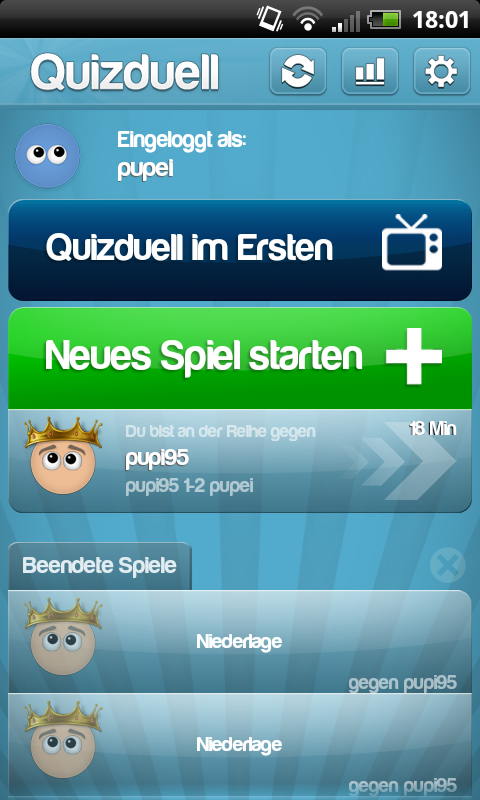
\includegraphics[scale=0.5]{Bilder/start.png}
\caption{Startbildschirm}
\end{figure}

Hier ist der Startbildschirm, nachdem man eingeloggt ist. Oben hat man die Funktionen Aktualisieren, Statistiken und Einstellungen. Beim Aktualisieren wird die Seite aktualisiert. \\

\begin{figure}[H]
\centering
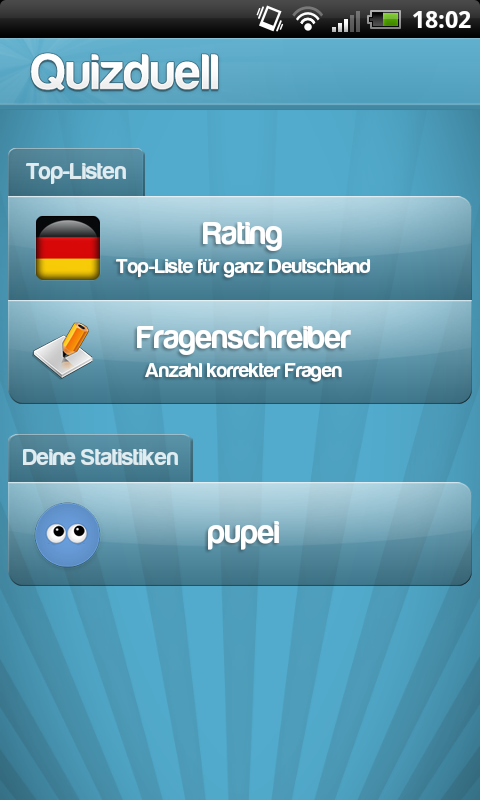
\includegraphics[scale=0.5]{Bilder/stat.png}
\caption{Statistiken}
\end{figure}

Hier kann man die Rating Liste aller Nutzer in Deutschland im Bezug auf der Punktzahl und der Anzahl der geschrieben und angenommenen Fragen sehen. Für die eigene Statistik wird eine Premium-Version benötigt.\\

\begin{figure}[H]
\centering
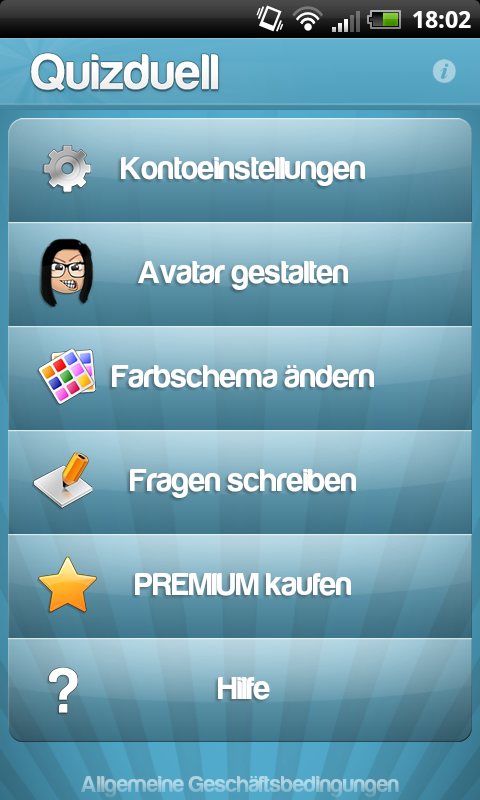
\includegraphics[scale=0.5]{Bilder/optionen.png}
\caption{Einstellungen}
\end{figure}

Unter Einstellungen kann man seine Kontoeinstellungen bearbeiten, wo man den Benutzernamen und Passwort ändern kann. Für Avatar gestalten und Farbschema ändern beötigt man die Premium-Version, welche man unter PREMIUM kaufen erwerben kann. Bei Fragen schreiben, kann man eigene Fragen schreiben, die evtl. dann übernommen werden. Bei Hilfe werden bestimmte Fragen im Hinblick auf die Benutzung beantwortet.\\

\begin{figure}[H]
\centering
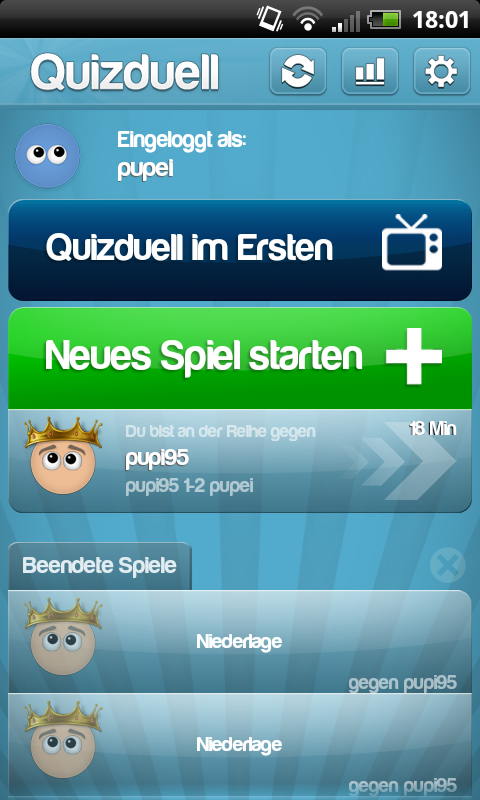
\includegraphics[scale=0.5]{Bilder/start.png}
\caption{Startbildschirm}
\end{figure}

Weitere Funktionen beim Startbildschirm sind Neues Spiel starten oder ein bereits angefangenes Spiel weiterspielen.\\

\begin{figure}[H]
\centering
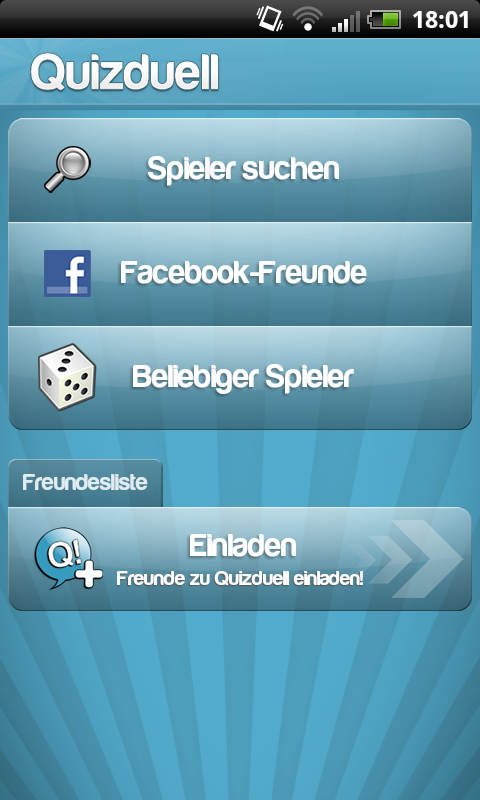
\includegraphics[scale=0.5]{Bilder/neuesspiel.png}
\caption{Bildschirm wenn man ein neues Spiel starten möchte}
\end{figure}

Wenn man ein neues Spiel starten möchte, kann man einen neuen Spieler suchen, unter Facebook Freunden suchen, falls man unter Facebook eingeloggt ist, oder gegen einen beliebigen Spieler spielen, der ebenfalls einen gesucht hat. 


\begin{figure}[H]
\centering
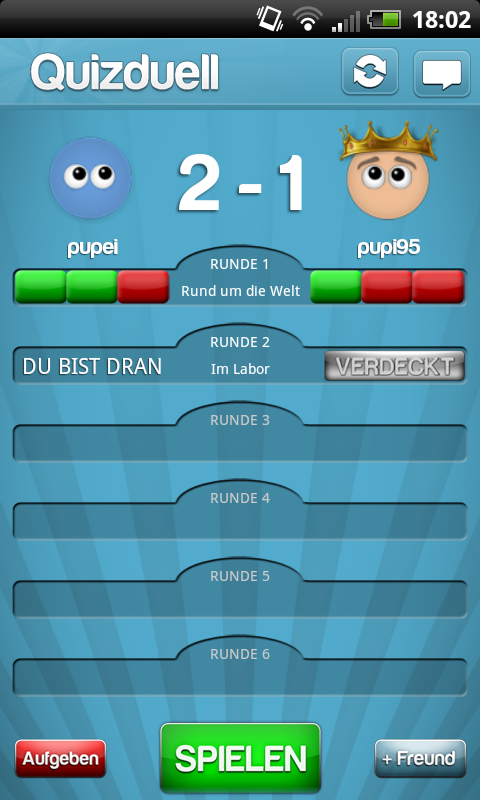
\includegraphics[scale=0.5]{Bilder/spiel.png}
\caption{Bildschirm beim neuen oder laufenden Spiel}
\end{figure}

Hier wird der bisherige Spielstand angezeigt. Insgesamt gibt es 6 Fragen, welche jeder beantworten muss. Die Spieler erhalten jeweils die gleichen Fragen. Es werden immer 2 Fragen abwechselnd gestellt, wobei der Spieler einmal eine Kategorie auswählen darf und einmal die Fragen der Kategorie des Gegners beantworten muss. Die Spieler haben 48 Stunden Zeit, die Fragen zu beantworten, bis das Spiel automatisch mit einer Niederlage des Spielers, der nicht geantwortet hat, endet. 

\begin{figure}[H]
\centering
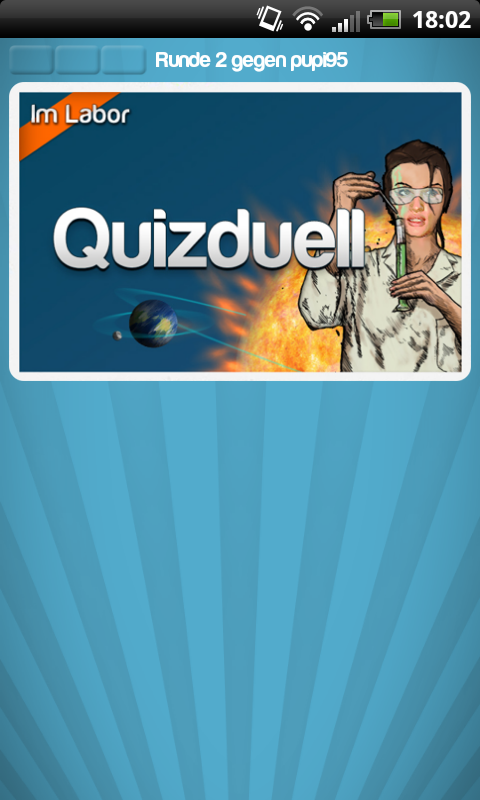
\includegraphics[scale=0.5]{Bilder/spielstart.png}
\caption{Beim Starten der Fragen}
\end{figure}

Beim Starten einer Frage erscheint erst nur eine Karte mit der Kategorie, bei einer Berührung wird die Karte umgedreht.\\

\begin{figure}[H]
\centering
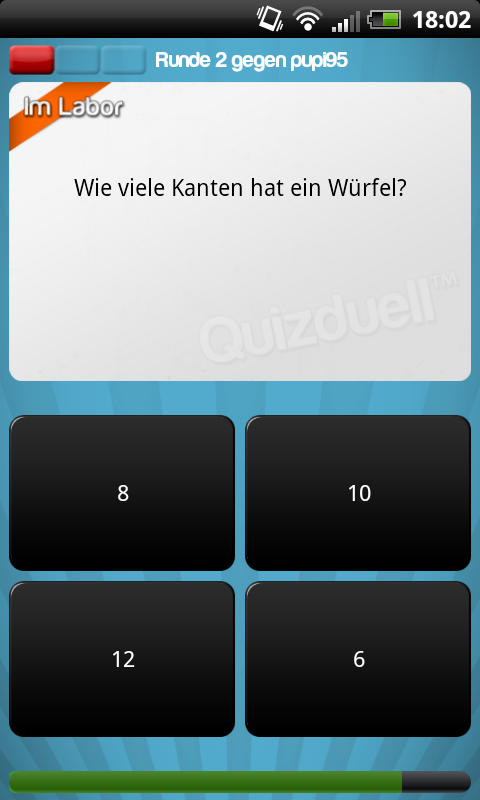
\includegraphics[scale=0.5]{Bilder/frage.png}
\caption{Anzeigen der Frage}
\end{figure}

Nun wird die Frage angezeigt, man hat 20 Sekunden Zeit, um die Frage zu beantworten, sonst wird diese als falsch gewertet.\\

\begin{figure}[H]
\centering
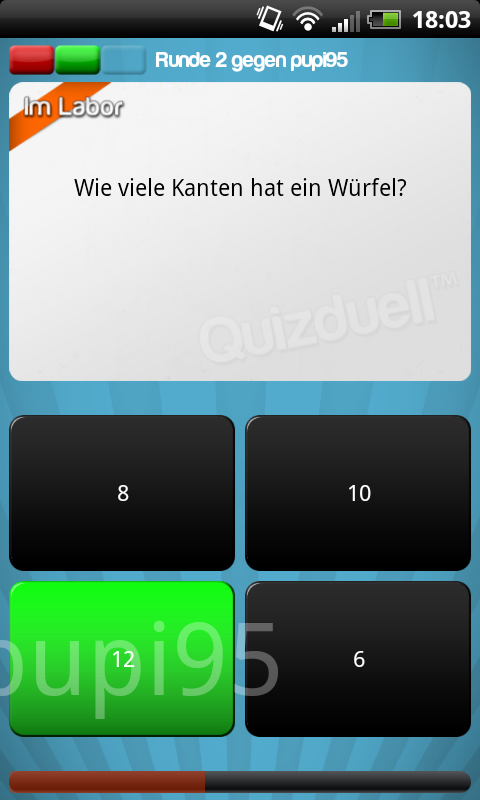
\includegraphics[scale=0.5]{Bilder/antwort.png}
\caption{Reaktion bei richtiger Antwort}
\end{figure}

Bei einer richtigen Antwort wird diese mit Grün unterlegt und zeitgleich wird der Name des Gegners auf seiner Antwort angezeigt, wenn er diese bereits beantwortet hat. Bei einer falschen wird die Antwort mit rot unterlegt.\\

\textbf{Fazit:}\\
Die \textit{Quizduell} App ist ein gutes System, mit welcher man unseres später vergleichen kann. Es hat viele Funktion, wie gezeigt, welche unser System ebenfalls haben muss. Es gibt allerdings auch Unterschiede. In unserer App wird es nur 3 Fragen pro Runde geben und es werden keine eigenen Fragen geschrieben, außerdem wird es keine Premium-Version geben. Zudem werden wir auch Offline-Funktion einbauen, in welcher der Spieler alleine spielen kann.\\ 

\subsection{Produktperspektive (Tim W. und Tim E.)}
  
\subsubsection{Systemschnittstellen}
  
Als Grundlage dient ein neu aufzusetzendes oder bestehendes System, auf dem die Software installiert werden kann. Als externe Schnittstelle muss dieses mit dem Internet verbunden sein. Der Server der Quizapp kann an einem PC über HTTP mit einem HTML5-unterstützenden Browser angesprochen werden. Mobiler Zugriff erfolgt auf Android-Geräten zudem mit einer eigenen App.

\subsubsection{Benutzerschnittstelle}

Die GUI der Website weist je nachdem, ob sich ein normaler Nutzer oder ein Admin anmeldet, unterschiedliche Funktionalitäten auf. 

\subsubsection{Hardwareschnittstellen}

Die HTML-Website ist plattform-unabhängig nutzbar. Smartphones mit kompatibler Android-Version (welche?) können die Quizapp nutzen.


\subsubsection{Softwareschnittstellen}

  \begin{tabular}{|l|l|l|l|}\hline
    \textbf{Name} & \textbf{Version} & \textbf{Hersteller} & \textbf{Quelle} \\\hline
    Java Runtime & 6 Update 37 & Oracle & \url{http://java.com} \\\hline
    JUnit & & & \\\hline
    libGDX &  &  & \\\hline
    Android & & & \\\hline
  \end{tabular}

\subsubsection{Kommunikationsschnittstellen}
  
Das System muss mit einer öffentlichen IP-Adresse und Domain von außen ansprechbar sein. Die Bandbreite sollte groß genug sein, um mehreren Nutzern parallel den Zugang zur Software zu gewähren, wobei jeder Nutzer einzeln nur eine sehr geringe Bandbreite benötigt.

\subsubsection{Speicherbeschränkung}


Die App wird voraussichtlich bis zu 30 MB Speicherplatz beziehen. (Arbeitsspeicher?)


\subsubsection{Operationen (Betriebsmodi)}

Wir unterscheiden zwischen dem normalen Betriebsmodus und einem Wartungsmodus, in dem z.B. Backups aufgespielt werden können. Während des Wartungsmodus ist kein öffentlicher Zugriff vorgesehen. Im normalen Betriebsmodus wird unterschieden zwischen Admins, registrierten Benutzern und Gästen. Jeder hat das Recht zu spielen, wobei registrierte Nutzer Vorteile wie Statistiken etc. genießen. Der Admin kann das System über die Website verwalten, z.B. Nutzernamen ändern. In der App ist kein Admin-Modus vorhanden.

\subsubsection{Möglichkeiten der lokalen Anpassung}
  
Es handelt sich bei dem System um ein lauffähiges Gesamtpaket. Es muss keine Datenbank o.Ä. eingerichtet werden. Lediglich eine IP-Adresse muss eingerichtet werden. Somit ist keine lokale Anpassung nötig.

\subsection{Anwendungsfälle (Daniel)}

\begin{itemize}
	\item \textbf{1. App starten}\\
	Die App wird gestartet. 
	\item \textbf{2. Offline-Modus starten}\\
	Die App wird im Offline-Modus gestartet. Keine Anmeldung und Internet Verbindung notwendig.
	\item \textbf{3. Benutzer registrieren}\\
	Benutzer registriert sich mit Benutzernamen und Passwort
	\item \textbf{4. Benutzer anmelden}\\
	Der Benutzer meldet sich mit Benutzernamen und Passwort an. Die Daten werden gespeichert, sodass kein nochmaliges anmelden nötig ist.
	\item \textbf{5. Benutzer abmelden}\\
	Benutzer wird abgemeldet und muss sich beim nächsten Start wieder anmelden.
	\item \textbf{6. Spielen(Offline)}\\
	Der Akteur spielt Offline.
	\item \textbf{7. Spielen(Online)}\\
	Es erscheint eine Auswahl zwischen Neues Spiel starten
	und es werden alle offenen Spiele angezeigt
	\item \textbf{8. Neues Spiel}\\
	Es erscheint eine Liste aller Spieler die Online sind.
	\item \textbf{9. Gegner herausfordern}\\
	Aus der Liste kann ein Spieler angeklickt und herausgefordert werden.
	\item \textbf{10. Offenes Spiel spielen}\\
	Eine neue Spielrunde wird gestartet, die erste Frage erscheint.
	\item \textbf{11. Einstellungen ändern}\\
	Unter Einstellungen kann der Benutzername und das Passwort geändert werden
	\item \textbf{12. Website wird aufgerufen}\\
	Website wird angezeigt.
	\item \textbf{13. Admin anmelden}\\
	Benutzer meldet sich als Admin an. Die Website ist nur für Administratoren verwendbar.
	\item \textbf{14. Admin abmelden}\\
	Benutzer meldet sich als Admin ab.
	\item \textbf{15. Frage hinzufügen}\\
	Eine neue Frage wird hinzugefügt
	\item \textbf{16. Frage bearbeiten}\\
	Eine vorhandene Frage wird bearbeitet
	\item \textbf{17. Frage löschen}\\
	Eine vorhandene Frage wird gelöscht
		\item \textbf{18. Frageliste importieren}\\
		Eine Liste an Fragen wird importiert
		\item \textbf{19. Frageliste exportieren}\\
		Eine Liste an Fragen wird importiert
	\item \textbf{20. User löschen}\\
	Bestimmter User wird gelöscht
	\item \textbf{21. Passwort ändern}\\
	User will sein Passwort ändern	
\end{itemize}

\subsection{Charakteristika der Benutzer (Tim W.)}
	\begin{tabular}{|p{7,5cm}|p{7,5cm}|}\hline
       \textbf{Name:} &  \textbf{Armin Admin}\\\hline
       Benutzertyp: & Administrator\\\hline
       Tätigkeit	& Redakteur\\\hline
       Wohnort & Uniallee, Bremen\\\hline
       Alter	 & 42\\\hline
       Motivation & System aufrecht erhalten\\\hline
       Aufgaben & Verwaltung und Systemwartung\\\hline
    \end{tabular}\\
        
    	\begin{tabular}{|p{7,5cm}|p{7,5cm}|}\hline
        \textbf{Name:} &  \textbf{Paul Neuling}\\\hline
       Benutzertyp: & Gelegenheitsspieler \\\hline
       Tätigkeit	& Student\\\hline
       Wohnort & Uniallee, Bremen\\\hline
       Alter	 & 19\\\hline
       Motivation & Etwas über die Uni lernen und Spaß haben\\\hline
    \end{tabular}\\
    
    	\begin{tabular}{|p{7,5cm}|p{7,5cm}|}\hline
        \textbf{Name:} &  \textbf{Klaus Zocker}\\\hline
       Benutzertyp: & Häufiger Spieler \\\hline
       Tätigkeit	& Student\\\hline
       Wohnort & Uniallee, Bremen\\\hline
       Alter	 & 23\\\hline
       Motivation & Will die Rangliste anführen\\\hline
    \end{tabular}\\
    
    \begin{tabular}{|p{7,5cm}|p{7,5cm}|}\hline
        \textbf{Name:} &  \textbf{Sabine Ohnenetz}\\\hline
       Benutzertyp: & Gelegenheitsspielerin \\\hline
       Tätigkeit	& Student\\\hline
       Wohnort & Uniallee, Bremen\\\hline
       Alter	 & 19\\\hline
       Motivation & Offline etwas spielen \\\hline
    \end{tabular}\\
    
    \textbf{Armin Admin}
    
    Text...
    
    \textbf{Paul Neuling}
    
    Text...
    
    \textbf{Klaus Zocker}
    
    Text...
    
    \textbf{Sabine Ohnenetz}
    
    Text...
  
  \subsection{Einschränkungen (Tim E.)}

Im Folgenden listen wir die Mindestanforderungen des Produkts auf, die nur mithilfe eines Logins bei StudIP einzusehen sind\footnote{\url{https://elearning.uni-bremen.de/scm.php?cid=2b323f34b16a84e8dce31dcdfc0be6ad\&show\_scm=4c88951a202b2543c96de2c8a476d471}}.

\textbf{Server:}
\begin{itemize}
\item SpielerInnen können sich beim Server registrieren
\item verwaltet eine Liste aller SpielerInnen
\item verwaltet die Fragekategorien, die Fragen und die Antworten sowie Belohnungen
\item SpielerInnen können sich beim Server als gerade spielbereit setzen und wieder entfernen
\item auf Anfrage wird aus der Liste der gerade spielbereiten SpielerInnen zufällig eine konkrete GegnerIn ermittelt
\item verwaltet laufende Spiele und archiviert diese
\begin{itemize}
\item TeilnehmerInnen
\item aktueller Punktestand
\item gestellte Fragen
\item gegebene Antworten
\end{itemize}
\end{itemize}
\begin{itemize}
\item verwaltet die Konfiguration der Spiele
\begin{itemize}
\item Anzahl Fragerunden
\item Anzahl Fragen pro Runde
\item Zeitspanne zur Auswahl einer Antwort
\item Punkte pro richtiger Antwort
\item Punkte für gewonnenes und unentschiedenes Spiel
\end{itemize}
\end{itemize}
\begin{itemize}
\item realisiert ein Belohnungssystem für SpielerInnen
\begin{itemize}
\item Erwerb eines Titels bei bestimmten Punktzahlen
\item Joker (z.B. Zeitverlängerung oder Anzeige der richtigen Antwort auf eine Frage)
\end{itemize}
\end{itemize}
\begin{itemize}
\item verwaltet eine Rangliste aller SpielerInnen
\item ein Spiel wird komplett vom Server geleitet, d.h. die Fragen und möglichen Antworten werden an die jeweiligen Clients gesendet und die korrekte Antwort wird vom Server geprüft (dies beinhaltet auch evtl. Spielregeln wie z.B. der Einsatz von Jokern oder das Einhalten der Zeitvorgaben)
\end{itemize}

\begin{itemize}
\item Administrationszugang über eine Webseite
\begin{itemize}
\item redaktionelle Bearbeitung der Fragen und Antworten
\begin{itemize}
\item Kategorien hinzufügen, Zuordnung der Fragen zu Kategorien ändern
\item Fragen und Antworten bearbeiten
\item Fragen und Antworten hinzufügen
\item Fragen und Antworten löschen
\end{itemize}
\item Import/Export der Fragen und Antworten in/aus geeignetem Format
\item Konfiguration der Spiele
\begin{itemize}
\item Anzahl Fragerunden
\item Anzahl Fragen pro Runde
\item Zeitspanne zur Auswahl einer Antwort
\item Punkte pro richtiger Antwort
\item Punkte für gewonnenes und unentschiedenes Spiel
\end{itemize}
\end{itemize}
\end{itemize}

\textbf{Client:}

\begin{itemize}
\item lauffähig auf Android-Systemen
\item unterstützt Registrierung und Anmeldung beim Server
\item neues Spiel starten
\item zufällige GegnerIn (siehe Server)
\item Auswahl einer GegnerIn aus Liste der spielbereiten SpielerInnen
\item Eingabe einer bekannten GegnerIn
\item eine Spielanfrage annehmen, d.h. an einem Spiel teilnehmen
\item Anzeige einer Frage mit möglichen Antworten
\item Auswahl einer Antwort in vorgegebener Zeitspanne
\item Anzeige einer Rangliste
\end{itemize}



\subsubsection{Technische Rahmenbedingungen} \label{subsubsec:TechRahmen} 
\begin{itemize}

\item Softwareergonomische Prinzipien werden umgesetzt
\item Der Server soll unter Linux, Windows und MacOS laufen (als Referenz gelten die Rechner in den Praktikumsräumen im MZH)
\item Es muss eine relationale Datenbank für die serverseitige Persistenz benutzt werden
\item Persistenz-Frameworks sind erlaubt (z.B. JPA)
\item Verwendung leichtgewichtiger DBMS (z.B. Derby, SQLite) ohne echte Serverinstallation ist vorgeschrieben
\item Verwendung und Abgabe eines Build-/Installationsskriptes, damit die Anwendung einfach installiert und aus den Quellen gebaut werden kann. Alle notwendigen Installations- und Konfigurationsschritte sind dokumentiert
\item Eventuell benutzte Fremdbibliotheken dürfen für den Einsatz in Forschung und Lehre keine Beschränkungen (Geld, Benutzung, ...) aufweisen
\item Quelltext in Deutsch oder Englisch dokumentiert. Gleiches gilt für Variablen- und Klassennamen. Alle anderen Dokumente in Deutsch
Die Implementierungssprache ist Java 6 oder höher (weitere zulässige Sprachen in geringem Umfang sind: HTML, XML und JavaScript)
\end{itemize}
	

\subsubsection{Gesetzliche Rahmenbedingungen} \label{subsubsec:GesetzlRahmen} Hier gilt in erster Linie das deutsche Recht. Um genau zu sein, kommen hier das Datenschutzgesetz\footnote{\url{http://www.gesetze-im-internet.de/bdsg_1990/}} und das Urheberrecht\footnote{\url{http://www.gesetze-im-internet.de/urhg/}} zum Tragen. Verfahrensrechtliche Vorkehrungen, um die Datensicherheit\footnote{\url{http://www.gesetze-im-internet.de/bdsg_1990/__9.html}} zu gewährleisten, sind von dem Kunden zu treffen. Der Kunde wird von der Software hinsichtlich der technischen Vorkehrungen insofern unterstützt, dass der Zugriff auf die Daten und der Zugang auf das Administrationstool passwortgeschützt ist. Hinsichtlich des Urheberrechts ist besonders auf die Regelung für Computerprogramme\footnote{\url{http://www.gesetze-im-internet.de/urhg/BJNR012730965.htm\#BJNR012730965BJNG004201377}} zu achten.

\subsubsection{Sicherheitskritische Aspekte} \label{subsubsec:SicherheitsAspekte} Um das deutschen Datenschutzgesetz einzuhalten, muss der Kunde weitere Maßnahmen treffen. Diese sind nicht entscheidend für die Entwicklung der Software und liegen in der Verantwortung des Kunden.

\subsection{Annahmen und Abhängigkeiten (Tim E.)} \label{subsec:Annahmen} Bis zur Auslieferung der Software wird sich der Kunde nicht ändern. Die Anforderungsspezifikation dient als eine Art Vertrag mit dem Kunden. Deshalb ist davon auszugehen, dass nach der Abgabe der Anforderungsspezifikation keine zusätzlichen Anforderungen hinzukommen. Abgabetermine haben Deadlines und sind somit strikt einzuhalten.\\
Des Weiteren wird davon ausgegangen, dass sich die Nutzer der Software zwar mit dem System eingehend auseinandersetzen. Es wird jedoch auch für den ungeübten Nutzer leicht möglich sein, dieses zu verwenden. Der jeweilige Nutzer sollte zumindest schon mal mit einem Computer bzw. Smartphone und dessen Bedienung vertraut sein.\\


\subsection{Ausblick (Tim E.)} \label{subsec:Ausblick} Große Änderungen sind nach Auslieferung des Systems zwar nicht zu erwarten, aber es können sich dennoch immer wieder mit der Zeit Anpassungen ergeben, die zu diesem Zeitpunkt allerdings noch nicht feststehen.

\section{Detaillierte Beschreibung}
\label{ch:DetaillierteBeschreibung}


\subsection{Datenmodell (Tobias)}

\subsubsection{Datenmodellbeschreibung}

Im Folgenden werden die einzelnen Klassen ergänzend beschrieben:

Nutzer:
Diese Einheit steht für den Appnutzung, die über verschiedene Aktionen
mit dem Serversystem in Verbindung steht. Die Einheit Nutzer hat sowohl 
alle Fragen als Stringliste, um auch offline spielen zu können,als auch 
den Usernamen gespeichert. 
Der Nutzer kann sich über das System einloggen, ausloggen oder auch erst noch 
registrieren.
Sobald sich der Nutzer angemeldet oder registriert hat, prüft das System automatisch,
ob die App auf dem neuesten Stand ist. Der Nutzer kann sowohl offline, als auch online 
über das System Spielen.

Server:
Die Klasse stellt die bereitgestellten Server und Datenbanken dar, indem alle 
nootwendigen Daten wie auch Quizfragen und Nutzerlisten gespeichert sind. Diese Einheit
steht abgesehen vom Offline-Spiel mit allen Aktionen der App oder Webseite in Verbindung.

Admin: 
Der Admin verwaltet das System oder die Server über eine bereitgestellte Webseite in der
sich einloggt oder wieder ausloggt. Er bearbeitet/löscht oder fügt Fragen hinzu, oder 
benennt gewisse Nutzer mit einem unangemessenen Nutzernamen um. Er kann einen Nutzer auch
löschen.

Bearbeiten/löschen/hinzufügen:
Diese Einheit stellt die Aktivitäten des Admin am Server dar. Der Admin kann eine Datei 
mit den neuen Fragen importieren und alles andere damit ersetzen oder einzelne löschen 
oder bearbeiten.

Update:
Das Update prüft mithilfe des Boolean isUpToDate, ob der eingeloggte Nutzer auf dem neusten Stand ist.
Dieser Boolean bekommt seinen Wert wiederrum mithilfe eines Vergleiches des letzten Einloggdatums des
Nutzers.

Einloggen/Ausloggen/Registrieren:
Der Einlogg- und der Registriervorgang ist sehr ähnlich, weshalb diese zusammengefasst wurden. 
Über diesen Vorgang wird die Gültigkeit des eingegebenen Passworts über den Nutzernamen verifiziert.
Sollte der Nutzer nach dem Verlassen der App nicht abgemeldet haben, so bleibt der Nutzer auch angemeldet
Daher wird in dieser Klasse nach dem Starten des OnlineModus der Boolean alreadyLoggedIn abgefragt.

Spielen.
Der Nutzer kann sowohl online, als auch offline spielen. Diese Einheit hat die/den Spieler
als Objekte und die Punkte der jeweiligen Spieler gespeichert. Es weiß auch,, welcher Spieler am Zug ist.
Am Ende eines Spiels wird der Gewinner in einem Boolean eingetragen.



\subsection{Anwendungsfälle (Tobias und Daniel)}

\begin{table}
	[H] \label{1} 
	\begin{tabular}
		{|l|p{10cm}|} \hline \textbf{1} & \textbf{App starten} \\
		\hline \textbf{Akteure} & Paul Neuling, Klaus Zocker, Sabine Ohnenetz\\
		\hline \textbf{Ziel} & Der Akteur möchte die App starten \\
		\hline \textbf{Vorbedingungen} & App bereits heruntergeladen und installiert \\
		\hline \textbf{Regulärer Ablauf} & 1. Der Akteur startet die App, indem er auf den Startbutton drückt \\
		&2. Die App startet und zeigt die Startseite \\
		\hline \textbf{Varianten} & keine \\
		\hline \textbf{Nachbedingungen} & Die App ist gestartet und der Benutzer kann diese nun verwenden\\
		\hline \textbf{Fehler-/Ausnahmefälle} & keine \\
		\hline 
	\end{tabular}
\end{table}

\begin{figure}
	[H] \caption{Startseite} 
	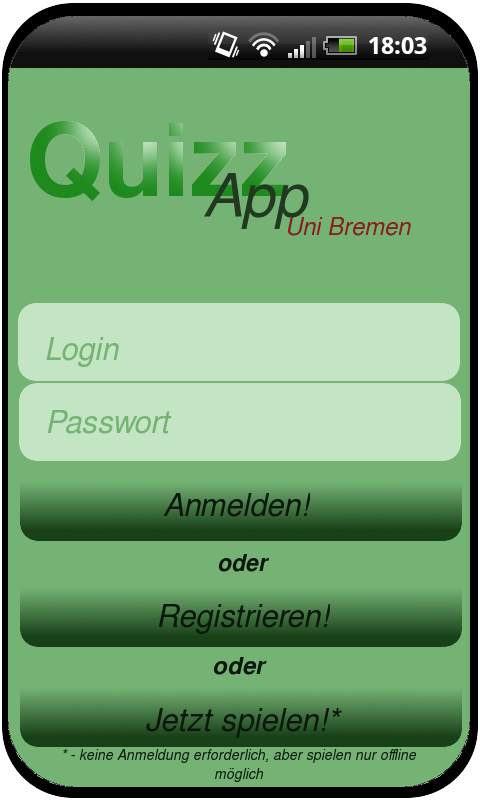
\includegraphics[width=0.5
	\textwidth]{Bilder/QuizzLoginRegister.png} \label{pic:Startseite} 
\end{figure}

\begin{table}
	[H] \label{2} 
	\begin{tabular}
		{|l|p{10cm}|} \hline \textbf{2} & \textbf{Offline-Modus starten} \\
		\hline \textbf{Akteure} & Paul Neuling, Sabine Ohnenetz\\
		\hline \textbf{Ziel} & Der Akteur möchte ohne Internet Verbindung und Anmeldung spielen \\
		\hline \textbf{Vorbedingungen} & App wurde bereits gestartet \\
		\hline \textbf{Regulärer Ablauf} & 1. Der Akteur drückt auf Jetzt Spielen \\
		\hline \textbf{Varianten} & keine \\
		\hline \textbf{Nachbedingungen} & Der Akteur kann nun ohne Anmeldung spielen\\
		\hline \textbf{Fehler-/Ausnahmefälle} & keine \\
		\hline 
	\end{tabular}
\end{table}

\begin{table}
	[H] \label{3} 
	\begin{tabular}
		{|l|p{10cm}|} \hline \textbf{3} & \textbf{Benutzer registrieren} \\
		\hline \textbf{Akteure} & Paul Neuling, Klaus Zocker\\
		\hline \textbf{Ziel} & Der Akteur möchte sich registrieren um im Internet gegen andere zu spielen \\
		\hline \textbf{Vorbedingungen} & App wurde bereits gestartet \\
		\hline \textbf{Regulärer Ablauf} & 1. Der Akteur drückt auf registrieren \\
		&2 Der Akteur gibt seinen Benutzernamen und Passwort an\\
		&3 Der Akteur drückt auf registrieren\\
		\hline \textbf{Varianten} & keine \\
		\hline \textbf{Nachbedingungen} & Der Akteur ist nun registriert und kann sich anmelden\\
		\hline \textbf{Fehler-/Ausnahmefälle} & 1. Es ist keine Internet-Verbindung vorhanden \\
		&2. Benutzername ist bereits vergeben\\
		&3. Doppelte Passworteingabe stimmt nicht überein\\
		\hline 
	\end{tabular}
\end{table}

\begin{table}
	[H] \label{4} 
	\begin{tabular}
		{|l|p{10cm}|} \hline \textbf{4} & \textbf{Benutzer anmelden} \\
		\hline \textbf{Akteure} & Paul Neuling, Klaus Zocker\\
		\hline \textbf{Ziel} & Der Akteur möchte sich anmelden und dann online spielen \\
		\hline \textbf{Vorbedingungen} & App wurde bereits gestartet \\
		\hline \textbf{Regulärer Ablauf} & 1. Der Akteur gibt seinen Benutzernamen und sein Passwort ein \\
		&2 Der Akteur drückt auf anmelden\\
		\hline \textbf{Varianten} & keine \\
		\hline \textbf{Nachbedingungen} & Der Akteur ist nun angemeldet und kann Online-Spielen\\
		\hline \textbf{Fehler-/Ausnahmefälle} & 1. Es ist keine Internet-Verbindung vorhanden \\
		&2. Benutzername existiert nicht\\
		&3. Passwort ist falsch\\
		\hline 
	\end{tabular}
\end{table}

\begin{table}
	[H] \label{5} 
	\begin{tabular}
		{|l|p{10cm}|} \hline \textbf{5} & \textbf{Benutzer abmelden} \\
		\hline \textbf{Akteure} & Paul Neuling, Klaus Zocker\\
		\hline \textbf{Ziel} & Der Akteur möchte sich abmelden\\
		\hline \textbf{Vorbedingungen} & Der Akteur war bereits angemeldet \\
		\hline \textbf{Regulärer Ablauf} & 1. Der Akteur drückt auf abmelden \\
		\hline \textbf{Varianten} & 1. Der Akteur ist bereits angemeldet, hat aber keine Internet-Verbindung und wird automatisch abgemeldet \\
		\hline \textbf{Nachbedingungen} & Der Akteur ist nun abgemeldet und ist wieder auf dem Startbildschirm\\
		\hline \textbf{Fehler-/Ausnahmefälle} & keine \\
		\hline 
	\end{tabular}
\end{table}

\begin{table}
	[H] \label{6} 
	\begin{tabular}
		{|l|p{10cm}|} \hline \textbf{6} & \textbf{Spielen(Offline)} \\
		\hline \textbf{Akteure} & Sabine Ohnenetz\\
		\hline \textbf{Ziel} & Der Akteur möchte spielen\\
		\hline \textbf{Vorbedingungen} & Der Akteur hat den Anwendungsfall 2 ausgeführt \\
		\hline \textbf{Regulärer Ablauf} & 1. Der Akteur drückt auf spielen \\
		\hline \textbf{Varianten} & keine \\
		\hline \textbf{Nachbedingungen} & Die Spielrunde wird gestartet\\
		\hline \textbf{Fehler-/Ausnahmefälle} & keine \\
		\hline 
	\end{tabular}
\end{table}


\begin{table}
	[H] \label{7} 
	\begin{tabular}
		{|l|p{10cm}|} \hline \textbf{7} & \textbf{Spielen(Online)} \\
		\hline \textbf{Akteure} & Paul Neuling, Klaus Zocker\\
		\hline \textbf{Ziel} & Der Akteur möchte spielen\\
		\hline \textbf{Vorbedingungen} & Der Akteur ist bereits Online angemeldet \\
		\hline \textbf{Regulärer Ablauf} & 1. Der Akteur drückt auf Spielen\\
		\hline \textbf{Varianten} & keine \\
		\hline \textbf{Nachbedingungen} & Es erscheint eine Auswahl zwischen Neues Spiel starten und es werden alle offenen Spiele angezeigt\\
		\hline \textbf{Fehler-/Ausnahmefälle} & keine \\
		\hline 
	\end{tabular}
\end{table}


\begin{table}
	[H] \label{8} 
	\begin{tabular}
		{|l|p{10cm}|} \hline \textbf{8} & \textbf{Neues Spiel} \\
		\hline \textbf{Akteure} & Paul Neuling, Klaus Zocker\\
		\hline \textbf{Ziel} & Der Akteur möchte ein neues Spiel starten\\
		\hline \textbf{Vorbedingungen} & Der Akteur hat bereits Anwendungsfall 7 ausgeführt \\
		\hline \textbf{Regulärer Ablauf} & 1. Der Akteur drückt auf neues Spiel \\
		\hline \textbf{Varianten} & keine \\
		\hline \textbf{Nachbedingungen} & Es wird eine Liste aller Spieler die Online sind angezeigt\\
		\hline \textbf{Fehler-/Ausnahmefälle} & Leere Liste, wenn keine Spieler online sind \\
		\hline 
	\end{tabular}
\end{table}

\begin{figure}
	[H] \caption{Liste aller Spieler die Online sind} 
	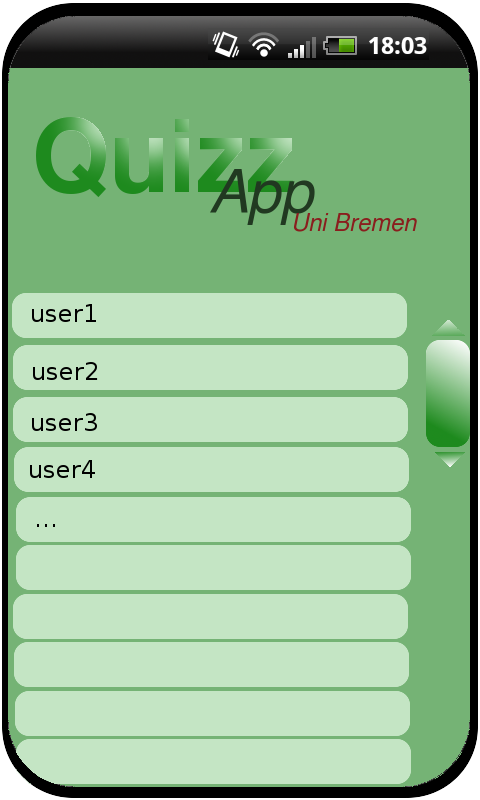
\includegraphics[width=0.5
	\textwidth]{Bilder/QuizzListeSpielerOnline.png} \label{pic:que} 
\end{figure}

\begin{table}
	[H] \label{9} 
	\begin{tabular}
		{|l|p{10cm}|} \hline \textbf{9} & \textbf{Gegner herausfordern} \\
		\hline \textbf{Akteure} & Paul Neuling, Klaus Zocker\\
		\hline \textbf{Ziel} & Der Akteur möchte einen anderen Spieler herausfordern\\
		\hline \textbf{Vorbedingungen} & Der Akteur hat bereits ein neues Spiel gestartet und eine Liste ist erschien(Anwendungsfall 8) \\
		\hline \textbf{Regulärer Ablauf} & 1. Der Akteur drückt in der Liste auf einen Spieler und fordert ihn heraus\\
		\hline \textbf{Varianten} & keine \\
		\hline \textbf{Nachbedingungen} & Es wird eine Anfrage an den Spieler gesendet und der Akteur kann bereits die erste Fragerunde beginnen\\
		\hline \textbf{Fehler-/Ausnahmefälle} & Leere Liste, wenn keine Spieler online sind \\
		\hline 
	\end{tabular}
\end{table}

\begin{table}
	[H] \label{10} 
	\begin{tabular}
		{|l|p{10cm}|} \hline \textbf{10} & \textbf{Offenes Spiel spielen} \\
		\hline \textbf{Akteure} & Paul Neuling, Klaus Zocker, Sabine Ohnenetz\\
		\hline \textbf{Ziel} & Der Akteur möchte anfangen die Fragen zu beantworten\\
		\hline \textbf{Vorbedingungen} & Der Akteur hat noch ein Spiel offen\\
		\hline \textbf{Regulärer Ablauf} & 1. Die erste Frage erscheint\\
		&2. Der Spieler hat 20sek Zeit die Frage zu beantworten\\
		&3. Nachdem der Spieler 3 Fragen weiter ist als der Gegner muss er warten\\
		\hline \textbf{Varianten} & Im Offline-Modus kann der Spieler so viele Fragen beantworten wie er will \\
		\hline \textbf{Nachbedingungen} & Der Akteur hat alle Fragen beantwortet und wartet nun auf den Gegner\\
		\hline \textbf{Fehler-/Ausnahmefälle} & keine \\
		\hline 
	\end{tabular}
\end{table}

\begin{figure}
	[H] \caption{Frage} 
	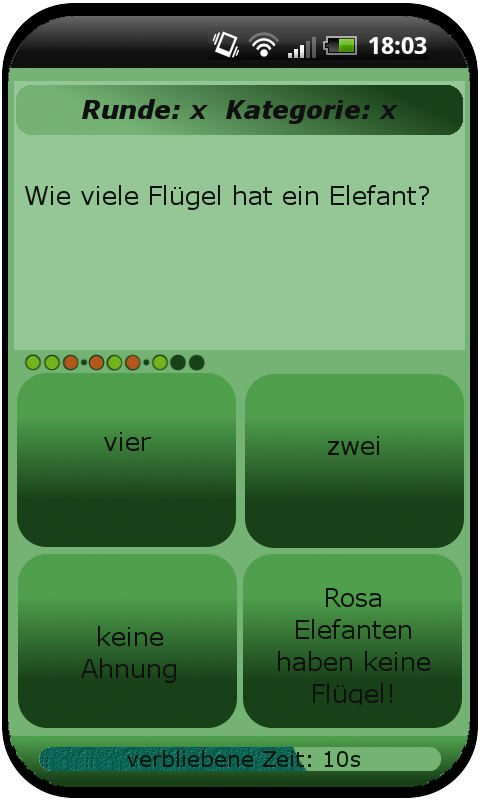
\includegraphics[width=0.5
	\textwidth]{Bilder/QuizzQuestion.png} \label{pic:ques} 
\end{figure}

\begin{table}
	[H] \label{11} 
	\begin{tabular}
		{|l|p{10cm}|} \hline \textbf{11} & \textbf{Einstellungen ändern} \\
		\hline \textbf{Akteure} & Paul Neuling, Klaus Zocker\\
		\hline \textbf{Ziel} & Der Akteur möchte seine Einstellungen ändern\\
		\hline \textbf{Vorbedingungen} & Der Akteur ist bereits angemeldet\\
		\hline \textbf{Regulärer Ablauf} & 1. Der Akteur gibt seinen neuen Nutzernamen an\\
		&2. Der Akteur gibt sein neues Passwort an\\
		\hline \textbf{Varianten} & keine \\
		\hline \textbf{Nachbedingungen} & Das Passwort und der Nutzername wurden geändert\\
		\hline \textbf{Fehler-/Ausnahmefälle} & Nutzername ist bereits vergeben \\
		\hline 
	\end{tabular}
\end{table}
\begin{table}
	[H] \label{12} 
	\begin{tabular}
		{|l|p{10cm}|} \hline \textbf{12} & \textbf{Website wird aufgerufen} \\
		\hline \textbf{Akteure} & Armin Admin\\
		\hline \textbf{Ziel} & Der Akteur will die Website aufrufen\\
		\hline \textbf{Vorbedingungen} & keine\\
		\hline \textbf{Regulärer Ablauf} & 1. Der Akteur ruft die Website auf, indem er die URL angibt\\
		\hline \textbf{Varianten} & keine \\
		\hline \textbf{Nachbedingungen} & Die Website wird angezeigt\\
		\hline \textbf{Fehler-/Ausnahmefälle} & Server nicht erreichbar \\
		\hline 
	\end{tabular}
\end{table}

\begin{table}
	[H] \label{13} 
	\begin{tabular}
		{|l|p{10cm}|} \hline \textbf{13} & \textbf{Admin anmelden} \\
		\hline \textbf{Akteure} & Armin Admin\\
		\hline \textbf{Ziel} & Der Akteur möchte sich anmelden\\
		\hline \textbf{Vorbedingungen} & Website ist aufgerufen\\
		\hline \textbf{Regulärer Ablauf} & 1. Der Akteur gibt seinen Nutzernamen und Passwort an\\
		&2. Der Akteur drückt auf anmelden\\
		\hline \textbf{Varianten} & keine \\
		\hline \textbf{Nachbedingungen} & Der Akteur ist angemeldet\\
		\hline \textbf{Fehler-/Ausnahmefälle} & Falscher Nutzername oder Passwort \\
		\hline 
	\end{tabular}
\end{table}

\begin{table}
	[H] \label{14} 
	\begin{tabular}
		{|l|p{10cm}|} \hline \textbf{14} & \textbf{Admin abmelden} \\
		\hline \textbf{Akteure} & Armin Admin\\
		\hline \textbf{Ziel} & Der Akteur möchte sich abmelden\\
		\hline \textbf{Vorbedingungen} & Der Akteur möchte sich abmelden\\
		\hline \textbf{Regulärer Ablauf} & 1. Der Akteur drückt auf abmelden\\
		\hline \textbf{Varianten} & keine \\
		\hline \textbf{Nachbedingungen} & Der Akteur ist abgemeldet\\
		\hline \textbf{Fehler-/Ausnahmefälle} & keine \\
		\hline 
	\end{tabular}
\end{table}

\begin{table}
	[H] \label{15} 
	\begin{tabular}
		{|l|p{10cm}|} \hline \textbf{15} & \textbf{Frage hinzufügen} \\
		\hline \textbf{Akteure} & Armin Admin\\
		\hline \textbf{Ziel} & Der Akteur möchte eine Frage hinzufügen\\
		\hline \textbf{Vorbedingungen} & Der Akteur ist angemeldet\\
		\hline \textbf{Regulärer Ablauf} & 1. Der Akteur gibt die Frage und die Antworten an\\
		&2. Der Akteur drückt auf speichern\\
		\hline \textbf{Varianten} & keine \\
		\hline \textbf{Nachbedingungen} & Die Frage wurde gespeichert\\
		\hline \textbf{Fehler-/Ausnahmefälle} & Frage, bzw. Antworten unvollständig ausgefüllt \\
		\hline 
	\end{tabular}
\end{table}

\begin{table}
	[H] \label{16} 
	\begin{tabular}
		{|l|p{10cm}|} \hline \textbf{16} & \textbf{Frage bearbeiten} \\
		\hline \textbf{Akteure} & Armin Admin\\
		\hline \textbf{Ziel} & Der Akteur möchte eine Frage bearbeiten\\
		\hline \textbf{Vorbedingungen} & Es existieren bereits Fragen\\
		\hline \textbf{Regulärer Ablauf} & 1. Der Akteur gibt die veränderte Frage und die Antworten an\\
		&2. Der Akteur drückt auf speichern\\
		\hline \textbf{Varianten} & keine \\
		\hline \textbf{Nachbedingungen} & Die alte Frage wurde gelöscht und die neue gespeichert\\
		\hline \textbf{Fehler-/Ausnahmefälle} & Frage, bzw. Antworten unvollständig ausgefüllt \\
		\hline 
	\end{tabular}
\end{table}

\begin{table}
	[H] \label{17} 
	\begin{tabular}
		{|l|p{10cm}|} \hline \textbf{17} & \textbf{Frage löschen} \\
		\hline \textbf{Akteure} & Armin Admin\\
		\hline \textbf{Ziel} & Der Akteur möchte eine Frage löschen\\
		\hline \textbf{Vorbedingungen} & Es existieren bereits Fragen\\
		\hline \textbf{Regulärer Ablauf} & 1. Der Akteur wählt die Frage aus\\
		&2. Der Akteur drückt auf löschen\\
		\hline \textbf{Varianten} & keine \\
		\hline \textbf{Nachbedingungen} & Die Frage wurde gelöscht\\
		\hline \textbf{Fehler-/Ausnahmefälle} & keine\\
		\hline 
	\end{tabular}
\end{table}

\begin{table}
	[H] \label{18} 
	\begin{tabular}
		{|l|p{10cm}|} \hline \textbf{18} & \textbf{Frageliste importieren} \\
		\hline \textbf{Akteure} & Armin Admin\\
		\hline \textbf{Ziel} & Der Akteur möchte eine Liste von Fragen importieren\\
		\hline \textbf{Vorbedingungen} & Es existiert bereits eine Liste von Fragen\\
		\hline \textbf{Regulärer Ablauf} & 1. Der Akteur wählt die Datei aus\\
		&2. Der Akteur drückt auf importieren\\
		\hline \textbf{Varianten} & keine \\
		\hline \textbf{Nachbedingungen} & Die Fragen wurden importiert\\
		\hline \textbf{Fehler-/Ausnahmefälle} & Falsches Dateiformat\\
		\hline 
	\end{tabular}
\end{table}


\begin{table}
	[H] \label{19} 
	\begin{tabular}
		{|l|p{10cm}|} \hline \textbf{19} & \textbf{Frageliste exportieren} \\
		\hline \textbf{Akteure} & Armin Admin\\
		\hline \textbf{Ziel} & Der Akteur möchte eine Liste von Fragen exportieren\\
		\hline \textbf{Vorbedingungen} & Es existieren bereits Fragen\\
		\hline \textbf{Regulärer Ablauf} & 1. Der Akteur drückt auf Datei exportieren\\
		&2. Der Akteur wählt den Speicherort aus\\
		\hline \textbf{Varianten} & keine \\
		\hline \textbf{Nachbedingungen} & Die Fragen wurden exportiert\\
		\hline \textbf{Fehler-/Ausnahmefälle} & keine \\
		\hline 
	\end{tabular}
\end{table}

\begin{table}
	[H] \label{20} 
	\begin{tabular}
		{|l|p{10cm}|} \hline \textbf{20} & \textbf{User löschen} \\
		\hline \textbf{Akteure} & Armin Admin\\
		\hline \textbf{Ziel} & Der Akteur möchte einen User löschen\\
		\hline \textbf{Vorbedingungen} & Der User existiert\\
		\hline \textbf{Regulärer Ablauf} & 1. Der Akteur drückt auf den entsprechenden User\\
		&2. Der Akteur drückt auf löschen\\
		\hline \textbf{Varianten} & keine \\
		\hline \textbf{Nachbedingungen} & Der User wurde gelöscht\\
		\hline \textbf{Fehler-/Ausnahmefälle} & keine \\
		\hline 
	\end{tabular}
\end{table}

\begin{table}
	[H] \label{21} 
	\begin{tabular}
		{|l|p{10cm}|} \hline \textbf{21} & \textbf{Passwort ändern} \\
		\hline \textbf{Akteure} & Armin Admin\\
		\hline \textbf{Ziel} & Der Akteur möchte sein Passwort ändern\\
		\hline \textbf{Vorbedingungen} & Der Akteur hat Einstellungen aufgerufen\\
		\hline \textbf{Regulärer Ablauf} & 1. Der Akteur gibt sein neues und altes Passwort an\\
		&2. Der Akteur drückt auf Passwort ändern\\
		\hline \textbf{Varianten} & keine \\
		\hline \textbf{Nachbedingungen} & Das Passwort wurde geändert\\
		\hline \textbf{Fehler-/Ausnahmefälle} & altes Passwort wurde falsch eingegeben \\
		\hline 
	\end{tabular}
\end{table}


\subsection{Aktionen (Tim W.)}
\subsubsection{App.Abmelden()}
\begin{itemize}
\item Der Nutzer meldet sich per Button ab.
\item \textbf{Vorbedingung}: Der Nutzer befindet sich im Online-Modus.
\item \textbf{Nachbedingung}: Der Nutzer kann zwischen Online- und Offline-Modus wählen. Beim nächsten Start wird der Nutzer nicht automatisch eingeloggt.
\item \textbf{max. Reaktionszeit}: 2 sek.
\end{itemize}

\subsubsection{App.Anmelden(nutzername, passwort)}
\begin{itemize}
\item Der Nutzer gibt seine Daten, mit denen er sich registriert hat, in zwei Eingabefelder ein und bestätigt die Eingabe mit einem Buttondruck.
\item \textbf{Vorbedingung}: Der Nutzer ist registriert und möchte den Onlinemodus starten. 
\item \textbf{Nachbedingung}: Der Nutzer ist eingeloggt und die Daten sind für den nächsten Start gespeichert.
\item \textbf{Fehlerbedingung}: Falls Nutzername oder Passwort nicht korrekt sind, wird der Nutzer aufgefordert, die Daten erneut einzugeben.
\item \textbf{max. Reaktionszeit}: 5 sek.
\end{itemize}

\subsubsection{App.Einstellungen ändern(neuerNutzername, neuesPasswort)}
\begin{itemize}
\item Der Nutzer kann im Einstellungsmenü einen neuen Nutzernamen und/oder ein neues Passwort bestimmen. Das neue Passwort muss durch eine zweite Eingabe in ein weiteres Eingabefeld bestätigt werden. Die Eingaben werden mit einem Buttondruck gespeichert.
\item \textbf{Vorbedingung}: Der Nutzer befindet sich im Einstellungsmenü.
\item \textbf{Nachbedingung}: Der Nutzer kehrt ins Menü zurück. Die Änderungen sind im Clienten und auf dem Server gespeichert.
\item \textbf{max. Reaktionszeit}: 3 sek.
\end{itemize}

\subsubsection{App.Einstellungen aufrufen()}
\begin{itemize}
\item Der Nutzer kann im Online-Modus per Button die Einstellungen aufrufen, um Nutzernamen oder Passwort zu ändern.
\item \textbf{Vorbedingung}: Der Nutzer befindet sich im Online-Modus.
\item \textbf{Nachbedingung}: Der Nutzer befindet sich im Einstellungsmenü. 
\item \textbf{max. Reaktionszeit}: 1 sek.
\end{itemize}

\subsubsection{App.Endergebnis bestätigen()}
\begin{itemize}
\item Nach einer Partie werden den Nutzern das Endresultat angezeigt. Um zum Menü zurückzukehren, drücken sie einen Button zur Bestätigung.
\item \textbf{Vorbedingung}: Eine Runde wurde beendet.
\item \textbf{Nachbedingung}: Der Nutzer kehrt ins Menü zurück. 
\item \textbf{max. Reaktionszeit}: 1 sek.
\end{itemize}

\subsubsection{App.Frage beantworten(antwort)}
\begin{itemize}
\item Der Nutzer beantwortet eine offene Frage, in dem er auf eine der vier Antwortmöglichkeiten drückt.
\item \textbf{Vorbedingung}: Eine Runde wurde gestartet.
\item \textbf{Nachbedingung}: Das System wertet die Antwort aus. Den Nutzern wird mitgeteilt, ob die Antwort stimmte. Die nächste Runde wird eingeleitet.
\item \textbf{max. Reaktionszeit}: 1 sek.
\end{itemize}

\subsubsection{App.Gegner herausfordern(nutzer)}
\begin{itemize}
\item Der Nutzer fordert einen Nutzer heraus, indem er auf einen der Namen in der Liste drückt. 
\item \textbf{Vorbedingung}: Der Nutzer startet ein Online-Match.
\item \textbf{Nachbedingung}: Die Herausforderung wurde versandt.
\item \textbf{Fehlerbedingung}: Falls die Übertragung fehlschlägt, wird dem Nutzer dies mitgeteilt.
\item \textbf{max. Reaktionszeit}: 3 sek.
\end{itemize}

\subsubsection{App.Herausforderung annehmen(herausforderung)}
\begin{itemize}
\item Der Nutzer lässt sich über einen Button offene Herausforderungen anzeigen und kann diese mit einem weiteren Druck annehmen. 
\item \textbf{Vorbedingung}: Der Nutzer ist im Online-Modus.
\item \textbf{Nachbedingung}: Die Herausforderung wurde angenommen und das Spiel wird gestartet.
\item \textbf{Fehlerbedingung}: Falls die Übertragung fehlschlägt, wird dem Nutzer dies mitgeteilt.
\item \textbf{max. Reaktionszeit}: 5 sek.
\end{itemize}

\subsubsection{App.Joker nutzen(art)}
\begin{itemize}
\item Der Nutzer nutzt einen Button, um während einer Fragerunde einen Joker zu nutzen.
\item \textbf{Vorbedingung}: Eine Runde wurde gestartet. Der Nutzer hat sich den Joker in einem früheren Spiel Joker erspielt.
\item \textbf{Nachbedingung}: Je nach Art des Jokers wird die Zeit verlängert oder zwei Antworten werden entnommen. 
\item \textbf{Fehlerbedingung}: Falls der Spieler bereits einen Joker gespielt hat, wird ihm mitgeteilt, dass er nicht noch einen spielen kann.
\item \textbf{max. Reaktionszeit}: 1 sek.
\end{itemize}

\subsubsection{App.Neues Spiel starten(modus)}
\begin{itemize}
\item Der Nutzer startet eine neue Partie per Button.
\item \textbf{Vorbedingung}: Der Nutzer befindet sich im Offline- oder Online-Modus.
\item \textbf{Nachbedingung}: Falls der Nutzer sich im Offline-Modus befindet, wird eine Einzelspieler Partie gestartet. Ist er online, wird ihm eine Liste von anderen Spielern angezeigt.
\item \textbf{Fehlerbedingung}: Falls keine weiteren Spieler online sind, wird dem Nutzer dies mitgeteilt und er kann es später noch einmal versuchen.
\item \textbf{max. Reaktionszeit}: 3 sek.
\end{itemize}

\subsubsection{App.Offline-Modus starten()}
\begin{itemize}
\item Der Nutzer wählt den Offline-Modus über einen Button aus.
\item \textbf{Vorbedingung}: Die App wurde gestartet.
\item \textbf{Nachbedingung}: Der Nutzer ist im Offline-Modus.
\item \textbf{max. Reaktionszeit}: 2 sek.
\end{itemize}

\subsubsection{App.Online-Modus starten()}
\begin{itemize}
\item Der Nutzer wählt den Online-Modus über einen Button aus.
\item \textbf{Vorbedingung}: Die App wurde gestartet.
\item \textbf{Nachbedingung}: Der Nutzer wird aufgefordert sich einzuloggen.
\item \textbf{Fehlerbedingung}: Falls der Server nicht angesprochen werden kann, wird dem Nutzer dies durch eine Fehlermeldung mitgeteilt.
\item \textbf{max. Reaktionszeit}: 1 sek.
\end{itemize}

\subsubsection{App.Rangliste aufrufen()}
\begin{itemize}
\item Der Nutzer kann im Online-Modus per Button die Rangliste aufrufen.
\item \textbf{Vorbedingung}: Der Nutzer befindet sich im Online-Modus.
\item \textbf{Nachbedingung}: Der Nutzer befindet sich im Ranglistenmenü. 
\item \textbf{max. Reaktionszeit}: 3 sek.
\end{itemize}

\subsubsection{App.Registrieren(nutzername, passwort)}
\begin{itemize}
\item Der Nutzer gibt seine Daten, mit denen er sich registrieren möchte, in zwei Eingabefelder ein und bestätigt die Eingabe per Button.
\item \textbf{Vorbedingung}: Die App ist gestartet.
\item \textbf{Nachbedingung}: Der Nutzer ist registriert.
\item \textbf{Fehlerbedingung}: Falls Nutzername oder Passwort nicht den Anforderungen entsprechen, wird der Nutzer an den entsprechenden Feldern darauf hingewiesen.
\item \textbf{max. Reaktionszeit}: 5 sek.
\end{itemize}


\subsubsection{Website.Anmelden(nutzername, passwort)}
\begin{itemize}
\item Der Admin gibt seine Daten, mit denen er sich einloggen möchte, in zwei Eingabefelder ein und bestätigt die Eingabe per Button.
\item \textbf{Vorbedingung}: Der Nutzer ist als Admin registriert.
\item \textbf{Nachbedingung}: Der Admin ist eingeloggt.
\item \textbf{Fehlerbedingung}: Falls Nutzername oder Passwort falsch sind, kann der Nutzer es nochmal probieren.
\item \textbf{max. Reaktionszeit}: 3 sek.
\end{itemize}

\subsubsection{Website.Abmelden()}
\begin{itemize}
\item Der Admin kann sich über das Menü abmelden.
\item \textbf{Vorbedingung}: Der Admin ist eingeloggt.
\item \textbf{Nachbedingung}: Der Admin ist ausgeloggt.
\item \textbf{max. Reaktionszeit}: 2 sek.
\end{itemize}

\subsubsection{Website.Frage bearbeiten(id, frage, antworten, kategorie)}
\begin{itemize}
\item Die Zellen der Fragenliste sind bearbeitbar. Der Admin kann an den nötigen Stellen einfach Änderungen vornehmen und mit einem Button bestätigen.
\item \textbf{Vorbedingung}: Der Admin hat die Fragenliste aufgerufen.
\item \textbf{Nachbedingung}: Die Änderungen wurden in der Datenbank eingetragen. Die Änderungen werden nun in der Liste angezeigt.
\item \textbf{max. Reaktionszeit}: 5 sek.
\end{itemize}

\subsubsection{Website.Frage hinzufügen(frage, antworten, kategorie)}
\begin{itemize}
\item Der Admin kann über einen Button ein Formular zum Hinzufügen einer neuen Frage aufrufen. Frage, Antworten und Kategorie werden in Eingabefelder eingetragen und per Button abgespeichert.
\item \textbf{Vorbedingung}: Der Admin hat die Fragenliste aufgerufen.
\item \textbf{Nachbedingung}: Die Frage wurde in der Datenbank eingetragen. Die Frage wird nun in der Liste angezeigt.
\item \textbf{Fehlerbedingung}: Falls etwas schief läuft, kann der Admin es nochmal probieren, die Daten im Formular gehen nicht verloren.
\item \textbf{max. Reaktionszeit}: 5 sek.
\end{itemize}

\subsubsection{Website.Frage löschen(id)}
\begin{itemize}
\item Die Zeilen der Fragenliste können markiert werden. Mehrere markierte Fragen können mit einem Buttondruck gelöscht werden, wobei dies mit einem weiteren Klick bestätigt oder abgebrochen werden kann.
\item \textbf{Vorbedingung}: Der Admin hat die Fragenliste aufgerufen.
\item \textbf{Nachbedingung}: Die markierten Fragen wurden gelöscht. Die Änderungen werden nun in der Liste angezeigt.
\item \textbf{Fehlerbedingung}: Falls etwas schief läuft, kann der Admin es nochmal probieren, die markierten Fragen bleiben weiterhin markiert.
\item \textbf{max. Reaktionszeit}: 5 sek.
\end{itemize}

\subsubsection{Website.Fragenliste aufrufen()}
\begin{itemize}
\item Der Admin kann über das Menü die Liste aller Fragen einsehen.
\item \textbf{Vorbedingung}: Der Admin ist eingeloggt.
\item \textbf{Nachbedingung}: Dem Admin wird die Fragenliste angezeigt. 
\item \textbf{max. Reaktionszeit}: 3 sek.
\end{itemize}

\subsubsection{Website.Nutzerliste aufrufen()}
\begin{itemize}
\item Der Admin kann über das Menü die Liste registrierter Nutzer einsehen.
\item \textbf{Vorbedingung}: Der Admin ist eingeloggt.
\item \textbf{Nachbedingung}: Dem Admin wird die Nutzerliste angezeigt. 
\item \textbf{max. Reaktionszeit}: 3 sek.
\end{itemize}

\subsubsection{Website.Nutzer löschen(id)}
\begin{itemize}
\item Die Zeilen der Nutzerliste können markiert werden. Mehrere markierte Nutzer können mit einem Buttondruck gelöscht werden, wobei dies mit einem weiteren Klick bestätigt oder abgebrochen werden kann.
\item \textbf{Vorbedingung}: Der Admin hat die Nutzerliste aufgerufen.
\item \textbf{Nachbedingung}: Die markierten Nutzer wurden gelöscht. Die Änderungen werden nun in der Liste angezeigt.
\item \textbf{Fehlerbedingung}: Falls etwas schief läuft, kann der Admin es nochmal probieren, die markierten Nutzer bleiben weiterhin markiert.
\item \textbf{max. Reaktionszeit}: 5 sek.
\end{itemize}

\subsubsection{Website.Nutzernamen ändern()}
\begin{itemize}
\item Der Admin kann jeden Nutzernamen in der Liste bearbeiten und die Änderungen mit einem Button abspeichern.
\item \textbf{Vorbedingung}: Der Admin hat die Nutzerliste aufgerufen.
\item \textbf{Nachbedingung}: Die Nutzernamen werden in der Datenbank geändert. Die Nutzerliste ist weiterhin aufgerufen.
\item \textbf{Fehlerbedingung}: Falls etwas schief läuft, kann der Admin es nochmal probieren, die aktuellen Änderungen bleiben in den Eingabefeldern erhalten.
\item \textbf{max. Reaktionszeit}: 5 sek.
\end{itemize}


\subsection{Softwaresystemattribute Tim E.)}
\label{sec:softwaresystemattribute}

  Hier werden die sogenannten „nichtfunktionalen Anforderungen“ spezifiziert. Dazu gehören beispielsweise: 
\begin{itemize}
	\item Performanz: Beim Entwickeln unserer Software wird Anspruch auf eine fließende Arbeitsweise gelegt, was bedeutet, dass Interaktionen mit dem System möglichst schnell zu bewältigen sind. Deshalb ist darauf zu achten, Berechnungsprozesse so wenig komplex wie möglich zu halten. Die Implementierung eines Ladezeichens bei aufkommenden Verbindungsschwierigkeiten ist selbstverständlich vorgesehen.
	
	\item Zuverlässigkeit (Korrektheit, Robustheit, Ausfallsicherheit): Die zu entwickelnde Software, insbesondere die Androidapplikation soll auf vielen verschiedenen Geräten funktionieren, weshalb trotz sorgfältig geplanten Testdurchläufe keine absolute Zuverlässigkeit garantiert werden kann. 
	
	\item Verfügbarkeit: Die Webapplikation soll wie gewohnt einfach über einen beliebigen Browser zugreifbar sein und die Androidappplikation soll auf jedem Gerät laufen, dass mit Android läuft und natürlich internetfähig ist. 
	
	\item Sicherheit: Sicherheit bezüglich der persönlichen Daten wird zum Teil durch den passwortgeschützten Login gewährleistet, wobei jeder Nutzer ein individuelles Passwort besitzt. Auf Profildaten haben nur der bestimmte eingeloggte Nutzer und der Admin Zugriff. Zusätzlich werden vor dem Versenden von Daten, diese via SSL verschlüsselt, was die Datensicherheit in unserem System garantiert.
	
	\item Wartbarkeit: Um eine gute Wartbarkeit zu gewährleisten, soll der Programmcode in Komponenten aufgeteilt werden, dessen Zuständigkeit klar definiert sein muss. Zusätzlich zu einer übersichtliche Programmstruktur, soll der Code sorgfältig und umfassend kommentiert werden.
	
	\item Portabilität: Da die Androidapplikation auf jedem androidfähigem Gerät laufen können soll, ist eine hohe Portabilität bereits gegeben. Durch Tests auf den verschiedensten Endgeräten kann die Applikation auf auf diesen absolut funktionstüchtig laufen. 
\end{itemize}






\end{document}
